\clearpage
\chapter{\textbf{Anwendung und Ergebnisse}}\label{kap5}
%\addtocontents{toc}{\vspace{0.8cm}}

\section{Feature Vektor}
Der Feature Vektor FV beschreibt das Ergebnis des Datensets nach der Vorverarbeitung.
Die benutzten Felder werden bei jedem Anwendungsfall zunächst vom Programmierer selbst gewählt.
Durch die o.g. Schritte ergibt sich eine Vielzahl an möglichen zusätzlichen Features,
um die das Datenset erweitert werden kann. Es muss also zunächst ermittelt werden, welche dieser möglichen
Features wirklich aussagekräftig sind, um den FV nicht unnötig zu überladen. \\
Einige Algorithmen geben nach dem Training 
Auskunft darüber, in welchem Maß ein Feature in die Berechnung des Labels einfließt. Somit wurden zur Wahl eines
FVs, der nach dem Training mit einem Modell eine möglichst hohe Genauigkeit liefert, verschiedene Kombinationen 
von möglichen Feldern durch Verknüpfung von Temperatur, Luftfeuchtigkeit, CO2 mit jeweiligen Delta- und Shiftwerten 
vorgenommen. Anschließend werden die Modellgenauigkeiten einzelner FVs miteinander verglichen.

Ziel war es, mit einem möglichst kleinen Vektor eine möglichst hohe Genauigkeit zu erreichen, da bei den meisten Algorithmen eine 
direkte Abhängigkeit zwischen Dauer der Berechnung und Dimensionalität des FV besteht. \\\\ 

In diesem Fall wurden die Feature Importances eines Random Forest genutzt, um Auskunft darüber zu erhalten, wie 
relevant bestimmte Felder für die Erwartungsberechnung sind. Diese werden errechnet, indem geprüft wird, wie viele
Datensätze des Sets bestimmte Knoten des Baumes erreichen. Wenn ein beliebiger Decision Tree eine große Menge
des Datensets allein über seinen rechten Teilbaum klassifizieren kann, werden die darin enthaltenen Knoten schwerer
gewichtet, da sie in einem höheren Maß in die endgültige Entscheidung einfließen.\\\\

Diese Eigenschaft wurde zur Ermittlung des FVs genutzt, indem verschiedene Modelle mit einem FV-Kandidaten trainiert
wurden und anschließend sowohl die Genauigkeiten, als auch die Feature Importances gegenübergestellt wurden.
Features mit geringer Relevanz wurden entfernt und die Modellgenauigkeiten erneut geprüft, um so über mehrere 
Iterationen hinweg einen FV zu finden, dessen Felder möglichst hohe Aussagekraft besitzen, während die Anzahl 
nötiger Felder möglichst gering ist.

\newpage
Hierzu wurden die Sensordaten zunächst um Delta- und Shiftwerte erweitert, um den Modellen die Möglichkeit zu geben
die aktuellen Werte den vorangegangenen Messungen gegenüberzustellen. Mit diesem FV wurde dann ein Random Forest
trainiert und dessen Feature Importances ausgewertet.

\begin{figure}[h]
    \centering
    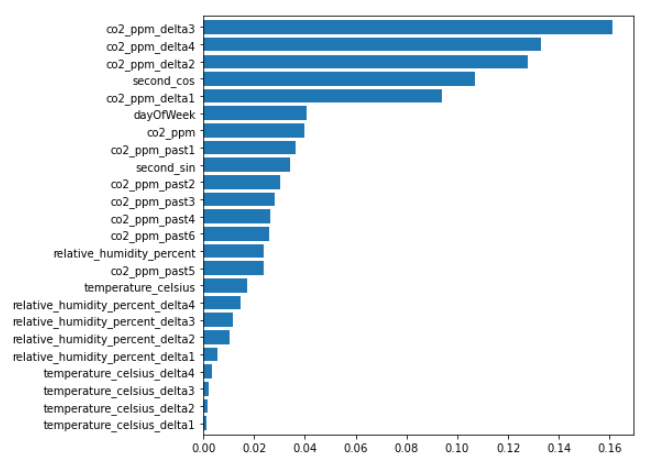
\includegraphics[width=0.8\textwidth]{pic/feature_importances.png}
    \caption{Feature Importances eines Random Forest}
    \label{fig:FI}
\end{figure}

Wie bereits im vorherigen Kapitel angedeutet, sieht man in Abb. \ref{fig:FI}, dass die Temperatur- und 
Luftfeuchtigkeitswerte für die Errechnung der Labels kaum zu Rate gezogen werden. 
Weder Grund- noch Deltawerte weisen eine hohe Relevanz für das Modell auf.\\
Es ist anzunehmen, dass Temperatur und Luftfeuchtigkeit an sich durchaus nützlich für solche Betrachtungen sein
können, allerdings werden sie durch die CO2-Werte in ihrer Relevanz übertroffen, da CO2 im Kontext menschlicher
Präsenz in Innenräumen eine deutlich höhere Aussagekraft besitzt.\\
%Zusätzlich weisen die Grundwerte Temperatur und Luftfeuchtigkeit über größere Zeiträume wetterbedingt starke 
%Schwankungen auf. Diese Schwankungen
%müssten von einem Modell zunächst von menschlicher Präsenz getrennt werden, da ein Temperaturanstieg nicht unbedingt
%Schlüsse auf Präsenz zulässt.\\
Die CO2-Werte sind für die Modelle einfacher zu klassifizieren. Die Messwerte
eines CO2-Sensors sind unabhängig von äußeren Einflüssen wie Jahreszeiten oder dem aktuellen Wetter 
und sind deshalb, wie in Abb. \ref{fig:FI} gezeigt, entscheidender Faktor bei der Berechnung.

\newpage

Nach anschließender Exkludierung von Temperatur und Luftfeuchtigkeit wurden neue Deltas und Shifts für die 
CO2-Werte eingefügt und die Feature Importances erneut betrachtet.

\begin{figure}[h]
    \centering
    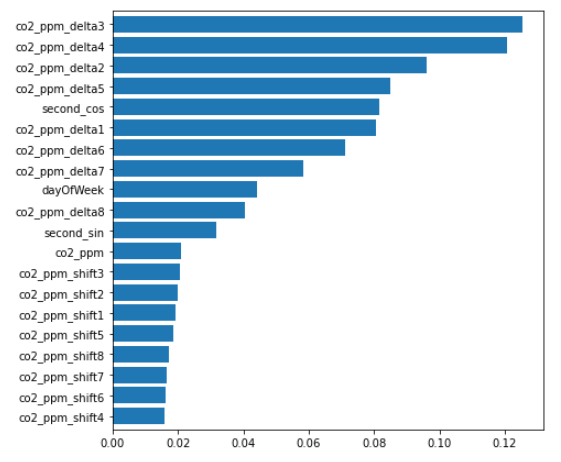
\includegraphics[width=0.9\textwidth]{pic/feature_importances_better.png}
    \caption{Feature Importances eines Random Forest}
    \label{fig:FIB}
\end{figure}

Es ist in Abb. \ref{fig:FIB} zu erkennen, dass die CO2-Shift-Werte ebenfalls nicht maßgeblich in die Berechnung einfließen. Diese weisen
allerdings noch deutlich höhere Feature Importances auf, als die Temperatur- und Luftfeuchtigkeitswerte.\\
Der Graph bestätigt die Annahme, dass beim CO2 die Deltawerte deutlich ausschlaggebender sind, als die 
tatsächliche Messung zu einem bestimmten Moment. \\

\newpage
Wenn diese Werte nur in solch geringem Maß zur Berechnung beitragen, muss ebenfalls die Schlussfolgerung daraus, 
dass die Genauigkeit auch ohne diese Werte innerhalb einer gewissen Toleranz konstant bleibt, überprüft werden.

Im Folgenden werden beispielhaft vier verschiedene Feature Vektoren beschrieben, aus denen der Vektor, der im 
weiteren Verlauf des Projektes benutzt werden sollte, abgeleitet wurde.
\begin{center}
    \begin{table}[h]
        \centering
        \caption{Vergleich Feature Vektoren}
        \begin{tabular}{ |c||c| } 
        \hline
        Feature Vektor & Beschreibung \\ 
        \hline\hline
        FV1 & CO2, Temperatur und Luftfeuchtigkeit mit Shift-Werten\\ 
        FV2 & CO2, Temperatur und Luftfeuchtigkeit ohne Shift-Werte \\ 
        FV3 & Nur CO2 mit Shift-Werten\\ 
        FV4 & Nur CO2 ohne Shift-Werte \\
        \hline
        \end{tabular}
    \end{table}
\end{center}

%\newpage
Mit diesen vier Vektoren wurden nun verschiedene Modelle trainiert und deren Genauigkeiten gegenübergestellt.

\begin{figure}[h]
    \centering
    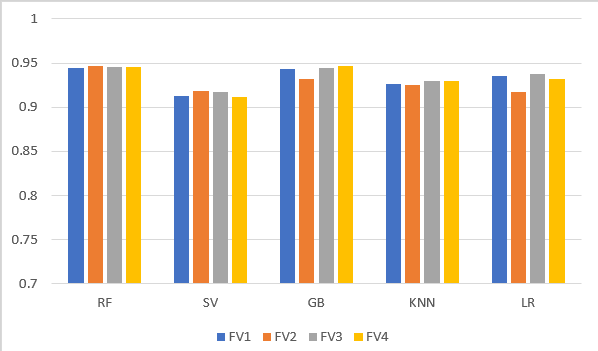
\includegraphics[width=0.8\textwidth]{pic/FV_comp.png}
    \caption{Vergleich der Genauigkeiten}
    \label{fig:FV_comp}
\end{figure}

Wie deutlich sichtbar ist, sind die Genauigkeiten fast identisch. Diese Gegenüberstellung wurde über das Projekt
hinweg mehrfach wiederholt und ergab immer ähnliche Unterschiede.\\
Dies war Anlass, sowohl die Temperatur- und Luftfeuchtigkeitswerte, als auch die Shift-Werte der CO2-Messungen 
nicht weiter zu betrachten, um den FV für Modelle mit hoher Empfindlichkeit gegenüber der Dimensionalität zu 
optimieren.

\newpage
Aus diesen Betrachtungen ergab sich folgender FV, der für den weiteren Verlauf des Projektes genutzt wurde:\\

\begin{center}
    \begin{table}[h]
        \centering
        \caption{Feature Vektor}
        \begin{tabular}{ |c||c| } 
        \hline
        Feld & Beschreibung \\ 
        \hline\hline
        second\_sin & timestamp-Sinusanteil\\
        second\_cos & timestamp-Cosinusanteil\\
        day\_of\_week & Wochentag der Messung\\
        co2\_ppm & CO2-Wert\\ 
        co2\_ppm\_delta1 & Delta zum CO2-Wert vor 2 Minuten\\ 
        co2\_ppm\_delta2 & Delta zum CO2-Wert vor 4 Minuten\\ 
        co2\_ppm\_delta3 & Delta zum CO2-Wert vor 6 Minuten\\ 
        co2\_ppm\_delta4 & Delta zum CO2-Wert vor 8 Minuten\\ 
        co2\_ppm\_delta5 & Delta zum CO2-Wert vor 10 Minuten\\ 
        co2\_ppm\_delta6 & Delta zum CO2-Wert vor 12 Minuten\\ 
        co2\_ppm\_delta7 & Delta zum CO2-Wert vor 14 Minuten\\ 
        co2\_ppm\_delta8 & Delta zum CO2-Wert vor 16 Minuten\\ 
        \hline
        \end{tabular}
    \end{table}
\end{center}

\newpage

\section{Ergebnisse}
%Da nicht alle Algorithmen auf die gleiche Weise evaluiert und grafisch dargestellt werden können, sollen 
%die Ergebnisse zu 
%\begin{itemize}
%    \item Decision Tree Modellen
%    \item Neuronalen Netzwerken
%    \item Clustering Modellen
%\end{itemize}
%einzeln betrachtet werden.

%\subsection{Decision Tree Modelle}
Die ausgewählten Algorithmen konnten mit dem ausgewählten FV bei der Erwartungsberechnung über das gesamte 
Datenset eine Genauigkeit von etwa 94\% erreichen.\\
Eine \textit{Confusion Matrix} (Abb. \ref{fig:ConMatrix}), welche die errechneten 
Werte den tatsächlichen Labelwerten gegenüberstellt, zeigt, dass im hier benutzten Beispiel ein Random Forest Classifier 
selbst bei der starken Unausgeglichenheit des Datensets ähnlich viele Fehler bei sowohl An- als auch Abwesenheit 
von Personen macht.\\
In den Feldern oben links und unten rechts ist jeweils zu sehen, wann das Modell eine richtige Erwartung 
für jeweils Ab- und Anwesenheit errechnet hat, während die Felder oben rechts und unten links jeweils die 
Menge falscher Erwartungen für beide Werte zeigen.

\begin{figure}[h]
    \centering
    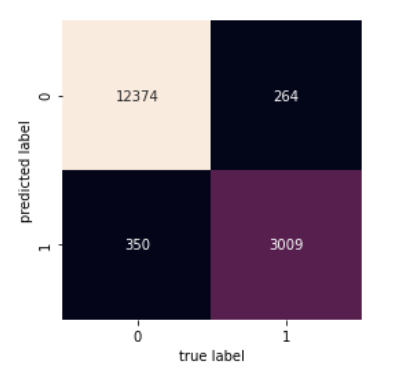
\includegraphics[width=0.5\textwidth]{pic/confusion_matrix.png}
    \caption{Confusion Matrix eines RFC}
    \label{fig:ConMatrix}
\end{figure}

Bezogen auf die Fehlerquote ist allerdings zu erkennen, dass die Berechnung von Abwesenheit mit wesentlich höherer
Genauigkeit erfolgt, als die Berechnung von Anwesenheit. In Abb. \ref{fig:ConMatrix} liegt die Genauigkeit Für
Abwesenheit etwa bei 97.5\%, während die Genauigkeit für Anwesenheit bei lediglich ca. 91.9\% liegt.
\\\\
Dies liegt daran, dass sehr viele Datenpunkte für Abwesenheit zwischen ca. 18:00 Uhr und
07:00 Uhr des nächsten Tages aufgezeichnet werden. Während dieser Zeit sind nie Personen anwesend, 
weshalb die Modelle diesen Teil des Datensets leicht klassifizieren können.\\
Während dem Arbeitstag zwischen ca. 07:00 Uhr und 17:00 Uhr existieren sowohl Messwerte für An- als auch für 
Abwesenheit, weshalb es hier deutlich schwieriger ist den richtigen Labelwert zu errechnen.\\\\
Dieser Trend lies sich bei allen Modellen beobachten. Die Genauigkeit bei der Errechnung von Abwesenheit
lag immer höher, als bei Anwesenheit.

\newpage

Die Gegenüberstellung der Durchschnittsgenauigkeiten aller Modelle mit Precision-, Recall- und F1-Scores in 
Abb. \ref{fig:ResAll}  zeigt, dass die Decision Tree Modelle bei diesem Klassifikationsproblem mit sehr hoher
Genauigkeit sowohl An-, als auch Abwesenheit berechnen können.
\begin{figure}[h]
    \centering
    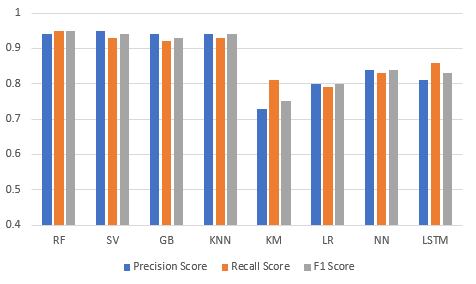
\includegraphics[width=0.7\textwidth]{pic/results_all.png}
    \caption{Durchschnittsgenauigkeiten aller Modelle}
    \label{fig:ResAll}
\end{figure}

Als Metrik wurde hier die Durchschnittsgenauigkeit der Genauigkeiten für An- und Abwesenheit gewählt, da die 
Datensets wie bereits beschrieben An- und Abwesenheit stark unausgeglichen sind. Wenn man die Genauigkeiten
nach der Menge der jeweiligen Datenpunkte gewichtet, erhöht das die Genauigkeit aller Modelle deutlich,
ohne dass sich deren Aussagekraft steigert.\\\\ 
Dieser Sachverhalt zeigt sich besonders deutlich durch die Darstellung der tatsächlichen Genauigkeiten bezogen 
auf die beiden Labelwertein Abb. \ref{fig:ResSpec}. Alle Modelle sind deutlich besser in der Erkennung von 
Abwesenheit.

\begin{figure}[h]
    \centering
    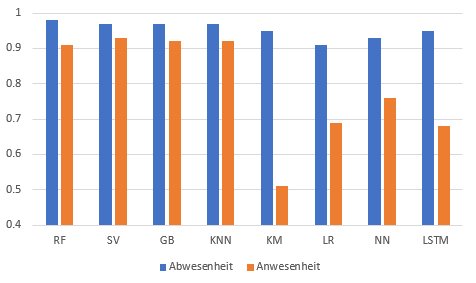
\includegraphics[width=0.7\textwidth]{pic/results_spec.png}
    \caption{Genauigkeiten einzelner Labelwerte aller Modelle}
    \label{fig:ResSpec}
\end{figure}

Besonders auffällig ist die niedrige Genauigkeit des K-Means Modells bei der Erkennung von Anwesenheit. Diese 
wird in \ref{KMeans} genauer betrachtet.
\newpage

Ebenfalls aufschlussreich, ist die grafische Gegenüberstellung der erwarteten Labelwerte mit den tatsächlichen Labelwerten
indem man das ursprüngliche Datenset mit \textit{timestamp} und \textit{CO2-Wert} zeichnet. Dabei markiert gelb 
die Anwesenheitund blau die Abwesenheit von Personen.

\begin{figure}[h]
    \centering
    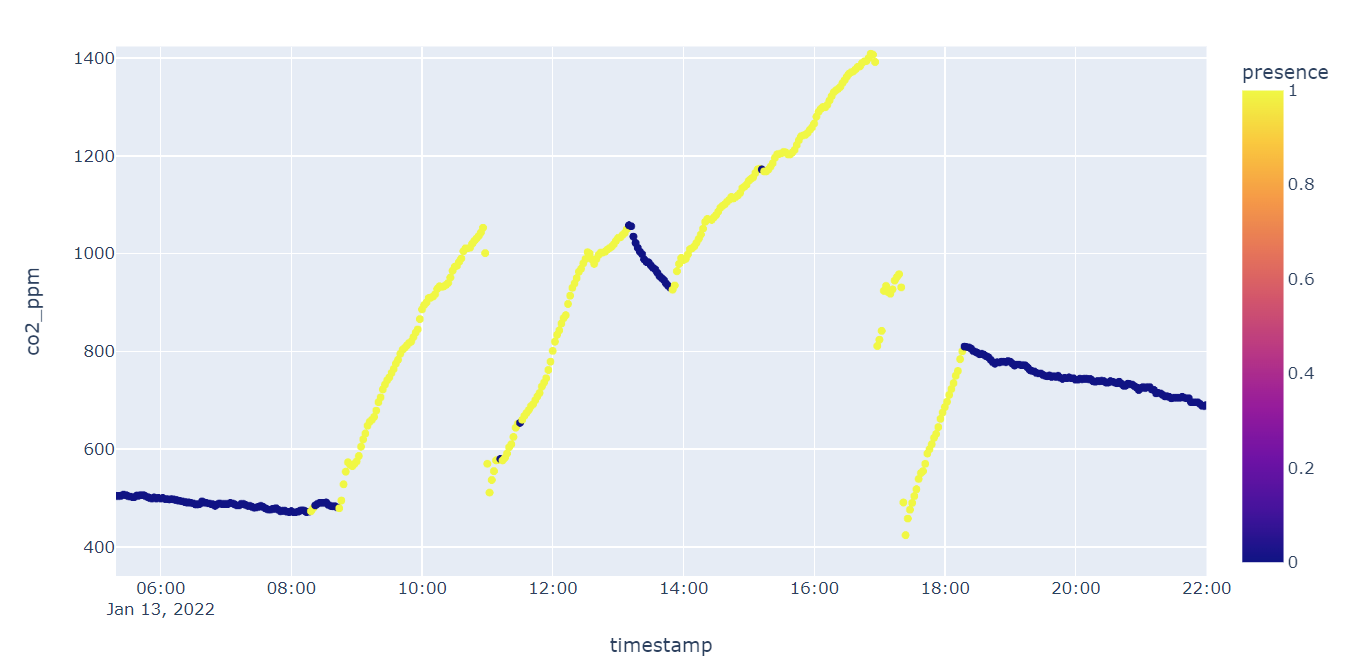
\includegraphics[width=0.9\textwidth]{pic/nov23_actual.png}
    \caption{Messwerte des 13. Januar}
    \label{fig:nov23}
\end{figure}

\ref{fig:nov23} zeigt den Verlauf der CO2-Messungen über einen Arbeitstag. Die blaue und gelbe Einfärbung stellt
die Messung des Infrarotsensors dar.\\ 
Ersetzt man aus dieser Datenreihe die tatsächlichen Messwerte des Infrarotsensors durch die errechneten 
Anwesenheitswerte des Modells, zeigt sich die hohe Genauigkeit in \ref{fig:nov23_pred} durch die neue Einfärbung 
der Datenreihe deutlich. 
Bis auf einige kleine Fehler trifft das Modell eine sehr präzise Aussage über die aktuelle Anwesenheit.

\begin{figure}[h]
    \centering
    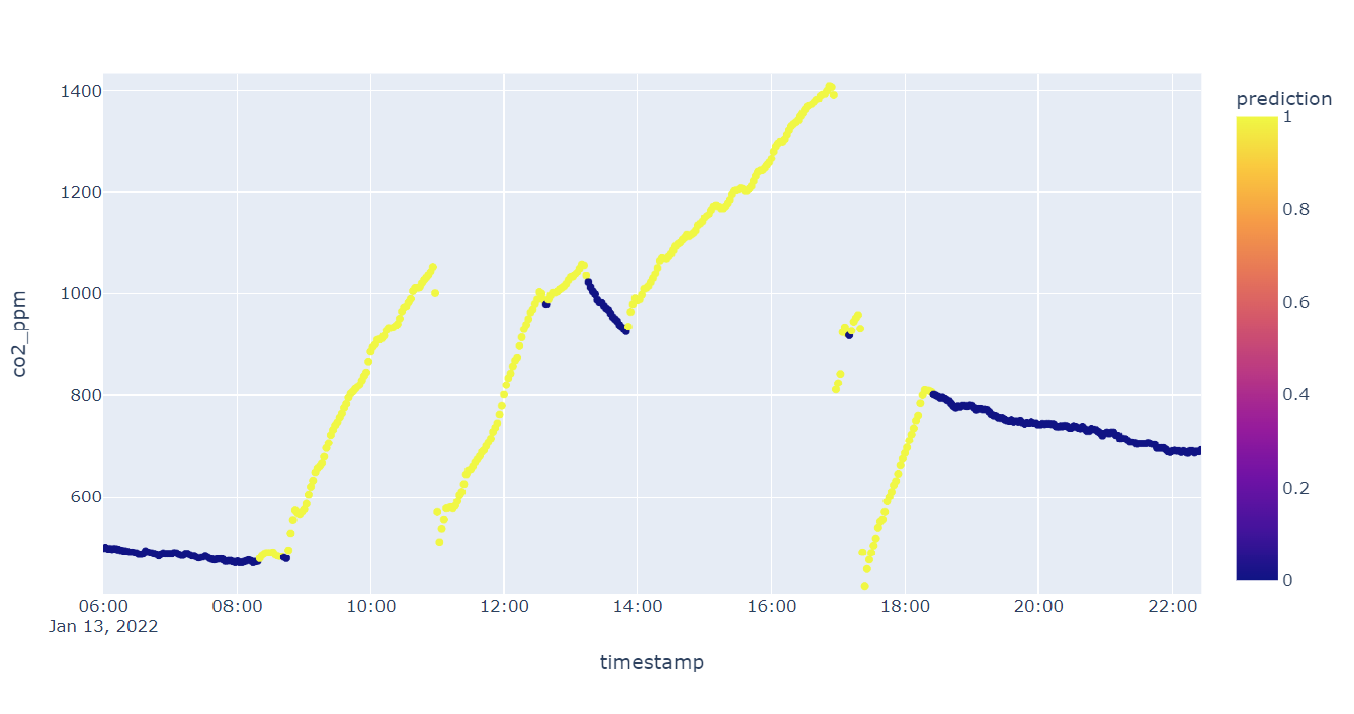
\includegraphics[width=0.9\textwidth]{pic/nov23_predicted.png}
    \caption{Erwartungsberechnung des 13. Januar}
    \label{fig:nov23_pred}
\end{figure}

Dieses Ergebnis konnte über weitere Kombinationen verschiedener Räume und Modelle weiterhin
bestätigt und repliziert werden. 

\newpage
%Die Tatsache, dass die Genauigkeiten aller Modelle so nah beieinander 
%liegen, rührt daher, dass dieses Datenset ein typisches Klassifizierungsproblem darstellt,
%wodurch die sich wiederholenden Schemata in den CO2-Werten von einer Vielzahl von Algorithmen schnell 
%erkannt und verarbeitet werden können.\\\\
Beim Parameter Tuning der ausgewählten Modelle wurden als Parameter-Optionen ausschließlich Werte gewählt, die nicht 
den Standardwerten der Modelle entsprechen. Somit sollte das GridSearchCV-Modul ausschließlich in der Menge 
von Parametern nach Möglichkeiten suchen, die nicht den Standard-Einstellungen entsprechen.\\
Hier ist anzumerken, dass das K-Means Modell kein Parameter Tuning unterstützt und deshalb hier nicht 
beachtet wird. Wie beschrieben, werden beim K-Means Algorithmus zufällige Datenpunkte in das Datenset
gelegt, weshalb nicht jede Ausführung des Modells die gleiche Genauigkeit liefert. Es ist deshalb auch
durch manuelle Veränderung der Parameter sehr schwer Verbesserungen der Genauigkeit herbeizuführen.\\
Neuronale Netze tauchen hier ebenfalls nicht auf, da diese Art von Modell vom GridSearchCV-Modul nicht
unterstützt wird. Die Layer des NN und LSTM wurden manuell erzeugt, wobei deren Anordnung bereits so
gewählt wurde, dass die Genauigkeiten möglichst maximiert werden.

\begin{figure}[h]
    \centering
    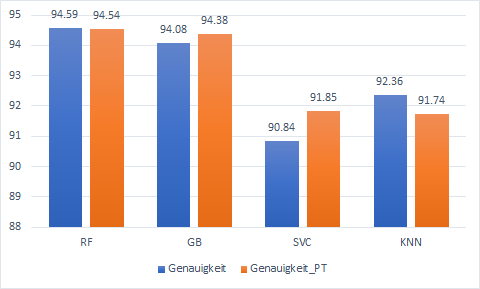
\includegraphics[width=0.6\textwidth]{pic/param_eval.png}
    \caption{Ergebnisse des Parameter Tuning}
    \label{fig:PT_eval}
\end{figure}

Es ist zu sehen, dass das Parameter Tuning die Genauigkeit der Modelle im erwarteten Rahmen erhöht oder 
verringert hat. Dies bestätigt die Annahme, dass dieser Anwendungsfall ein typisches Klassifizierungsproblem 
darstellt, weshalb die Modelle nicht mehr maßgeblich verbessert werden können. Der Schritt des Parameter Tunings 
sollte trotzdem grundsätzlich immer durchgeführt werden, um zu erkennen, ob man durch eine einfache Änderung 
der Parameter eine Verbesserung des Modells erzielen kann.\\

\newpage
Zusätzlich wurden die \textit{ROC-Curves} (ROC: englisch für \textit{receiver operating characteristic} 
bzw. deutsch Operationscharakteristik) gezeichnet, um zu erkennen, inwiefern die Ergebnisse zufällig 
oder errechnet sind.\\
Hierbei berechnet sich die True Positive Rate auf der y-Achse aus
\begin{align}
    \dfrac{TP}{TP - FN}
\end{align}
während die False Positive Rate auf der x-Achse durch
\begin{align}
    \dfrac{FP}{FP + TN}
\end{align}
angegeben wird.\\
Der Optimalwert wird hier durch in der grünen Kurve gezeigt, welche den Fall darstellt, 
dass das Modell die Labels immer richtig berechnet und es nie zu Fehleinschätzungen kommt.\\
Liegt ein Modell näher an der schwarzen Diagonale in der Mitte bedeutet das, dass True- und 
False-Positives jeweils 50\% der Ergebnismenge ausmachen. 
Das Modell liegt dann genauso oft richtig, wie es Fehleinschätzungen trifft. 
Je näher die einzelnen Modelle an der schwarzen Linie liegen, desto weniger aussagefähig sind sie. 

\begin{figure}[!h]
    \centering
    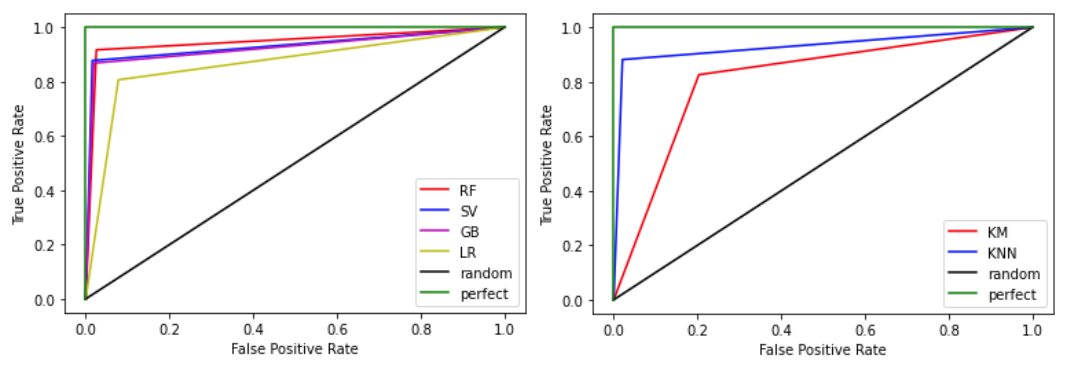
\includegraphics[width=0.9\textwidth]{pic/roc_all.png}
    \caption{ROC-Curves der Decision Tree und Clustering Modelle}
    \label{fig:Roc_curves}
\end{figure}
In \ref{fig:Roc_curves} ist zu sehen, wie alle Modelle sehr ähnliche Ergebnisse aufweisen. Keines der Modelle weist Anzeichen 
dafür auf, dass Ergebnisse wegen Underfitting erraten werden. Alle Modelle zeigen eine hohe Rate von True-Positives und
sind somit in den meisten Fällen in der Lage, aus den Input-Werten das richtige Ergebnis für die Präsenz abzuleiten.\\
Es ist auch zu erkennen, dass für diesen Anwendungsfall Decision Tree Modelle am besten abschneiden.
Von den Clustering Modellen ist das K-Nearest-Neighbours Modell erheblich genauer als das K-Means Modell. 
\newpage

\subsection{Umgang mit fehlenden Präsenz-Labels}
Da zur Auswertung auch eine große Menge an Datensätzen ohne Präsenz-Label zur Verfügung stand, konnte die 
Qualität der Ergebnisse für diese Datensets nicht rechnerisch quantifiziert werden. Die Ergebnisse
sind hierbei aufgrund der fehlenden Label lediglich augenscheinlich zu bewerten, da eine mathematische
Berechnung der Genauigkeit nicht möglich ist.\\
In diesem Kontext stellt sich die Frage, inwiefern ein auf einen Büroraum trainiertes Modell auch richtige
Erwartungen für einen Wohnraum treffen kann.
Da das Modell unter anderem auf eine Erkennung der aktuellen Tageszeit trainert wird, muss geprüft
werden, inwiefern ein solches Modell auch Aussagen über CO2-Werte treffen kann, dessen Veränderungen außerhalb
der bisher trainierten Arbeitszeiten von etwa 7 Uhr morgens bis 17 Uhr nachmittags liegen. 
Außerdem ist der Wohnraum in der Regel deutlich größer als ein Büro und weist in diesem Fall eine größere Anzahl 
anwesender Personen auf, wodurch sich die ermittelten Deltas der CO2-Werte erheblich von denen der Büroräume 
unterscheiden.
\newpage
Eines der Datensets zeichnete kontinuierliche Werte aus einem Wohnzimmer auf, in dem sich über einen 
Tag hinweg maximal drei Personen befanden. Die Zeiträume, zu denen in diesem Wohnzimmer anhand der CO2-Werte
Anwesenheit zu erkennen war, unterschieden sich deutlich von denen der Datensets der FH Aachen. Die 
starken Anstiege des CO2-Wertes waren bei diesem Datenset viel mehr über den Tag verteilt, wodurch sich die 
Datenreihe für diesen Test besonders anbot.\\
Auf dieses Datenset wurde das auf die Büroräume trainierte  SVC Modell angewendet, da dieses bisher die 
besten Ergebnisse bei der Unterscheidung von An- und Abwesenheit während eines Arbeitstages liefern konnte. 

\begin{figure}[h]
    \centering
    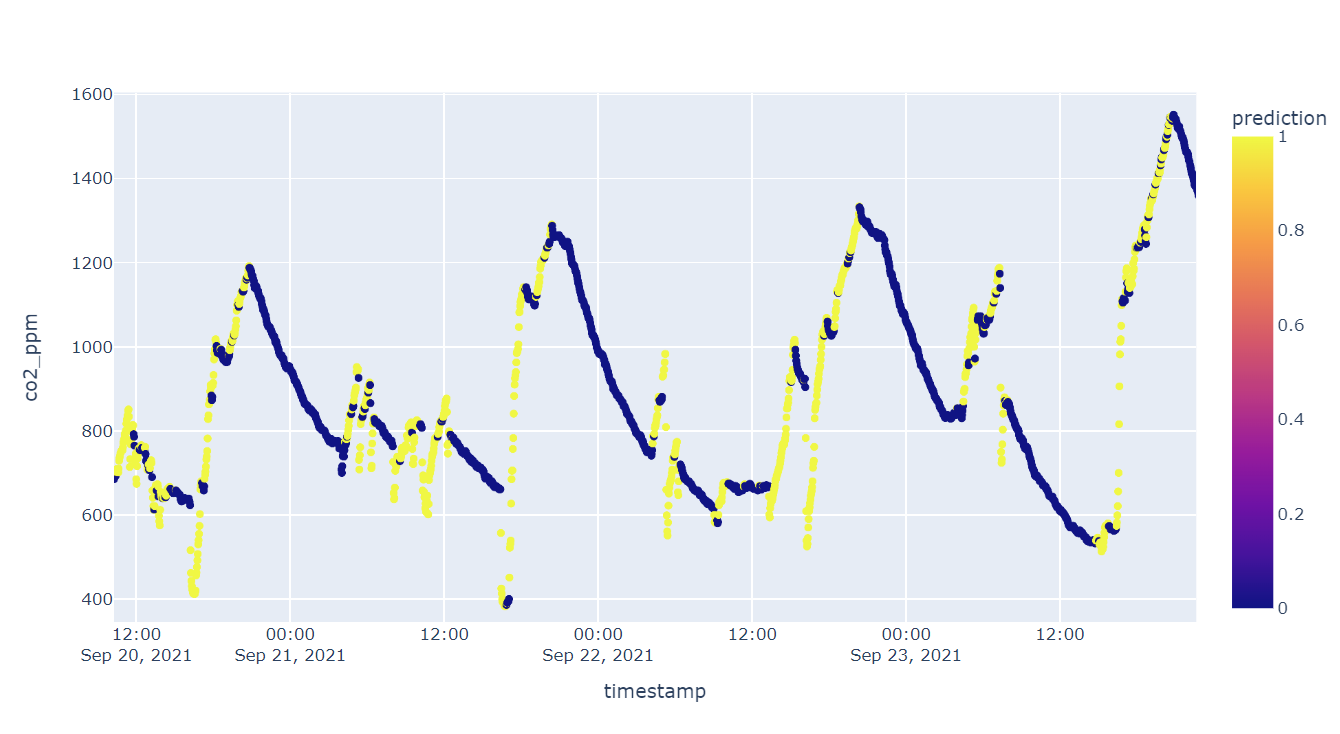
\includegraphics[width=0.95\textwidth]{pic/h217_predicting_livingroom.png}
    \caption{Büroraum-Modell trifft Erwartungen für Wohnzimmer}
    \label{fig:pred_livingroom}
\end{figure}

Auch hier wurden mit den errechneten Anwesenheitswerten des SVC Modells die Einfärbungen der einzelnen Datenpunkte 
vorgenommen. 
Wie in \ref{fig:pred_livingroom} anhand der Einfärbung zu erkennen ist, liegt die Vermutung nahe, dass das Modell 
auch unabhängig von der Tageszeit und den bekannten Gegebenheiten eines normalen Arbeitstages Anwesenheit 
erkennen kann. Vor allem deutliche Anstiege und Abfälle zeigen sich merklich durch kontinuierliche gelbe bzw. 
blaue Einfärbung.
\newpage

\subsection{Neuronale Netzwerke}
Die beiden implementierten neuronalen Netze konnten eine ähnliche Leistung wie die bereits oben genannten 
Algorithmen erzielen. Beide Modelle wurden über so viele Iterationen (Epochen) trainiert, bis ersichtlich war,
dass die Genauigkeit gegen einen Wert konvergiert. Zur Auswertung wurden hier die \textit{Accuracy-} und 
\textit{Loss}-Funktionen genutzt. Die Genauigkeit beschreibt wie bei den anderen Modellen das Verhältnis
zwischen richtigen und falschen Berechnungen.\\
Die Loss-Funktion hingegen gibt die Abweichung einer Schätzung zum tatsächlichen Wert an. Diese beiden Werte 
werden nach jeder Epoche ausgewertet, wobei zunächst der Erfolg während des Trainigs als \textit{train}
angegeben wird und danach das Modell an einem zufälligen Teil des Validierungssets \textit{val} getestet wird.
Liegen diese beiden Kurven nah beieinander, kann dies als ein klares Anzeichen für ein funktionierndes Modell ohne 
Over- oder Underfitting gewertet werden, da sowohl beim Training als auch bei der Validierung die Genauigkeiten 
Ähnlichkeiten aufweisen, während zugleich die Loss-Funktion minimiert wird.

\begin{figure}[h]
    \centering
    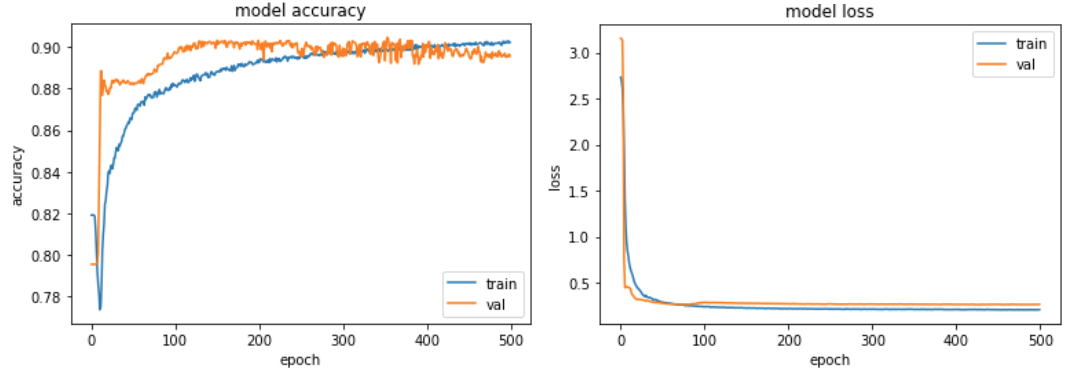
\includegraphics[width=0.9\textwidth]{pic/eval_NN.png}
    \caption{Ergebnisse des NN}
    \label{fig:eval_NN}
\end{figure}

\begin{figure}[h]
    \centering
    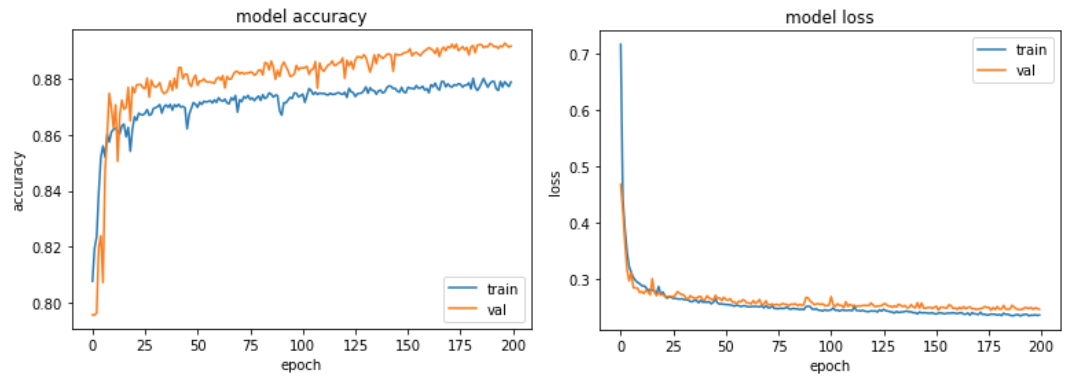
\includegraphics[width=0.9\textwidth]{pic/eval_LSTM.png}
    \caption{Ergebnisse des LSTM}
    \label{fig:eval_LSTM}
\end{figure}

Wie \ref{fig:eval_NN} und \ref{fig:eval_LSTM} zeigen, weisen beide Arten neuronaler Netzwerke diese Eigenschaften auf. Die Genauigkeiten beider Modelle
konvergierten auch nach verschiedenen Epochen-Werten etwa bei 89\%.

\newpage
Die ROC-Curves zeigen auch hier, dass die durchschnittliche Modellgenauigkeit nicht als Metrik ausreicht, um
die Qualität eines Modells festzustellen. Bei diesen Modellen zeigen sich deutlich größere Abweichungen zwischen
den Genauigkeiten für die Berechnung von Ab- und Abwesenheit. Wie in Abb. \ref{fig:Roc_nn} zu sehen, liefern
beide Modelle hohen Genauigkeiten bei der Errechnung von Anwesenheit.

\begin{figure}[!h]
    \centering
    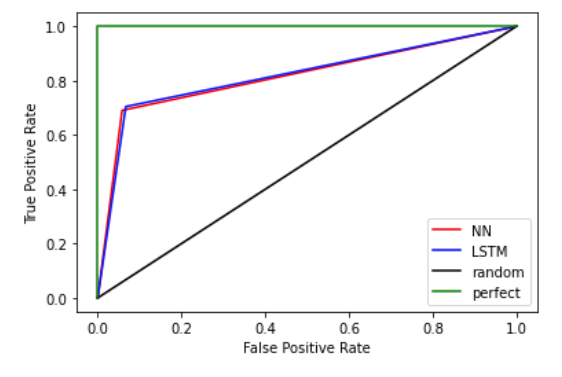
\includegraphics[width=0.6\textwidth]{pic/roc_nn.png}
    \caption{ROC-Curves aller Modelle}
    \label{fig:Roc_nn}
\end{figure}

Zieht man den Classification Report in Tab. \ref{tab:nn} hinzu, wird dieser Sachverhalt noch deutlicher.


\begin{table}[h]
    \centering
    \caption{Genauigkeitsauswertung des NN}
    \begin{tabular}{|p{2.5cm}||p{1.8cm}|p{1.5cm}|p{1.5cm}|}
        \hline
        \hfill Präsenz&\hfill Precision &\hfill Recall &\hfill F1\\
        \hline
        \hline
        \hfill Abwesenheit&\hfill 0.96&\hfill 0.92&\hfill 0.94\\
        \hfill Anwesenheit&\hfill 0.74&\hfill 0.83&\hfill 0.78\\
        \hline
    \end{tabular}          
    \label{tab:nn}
\end{table}
\begin{table}[h]
    \centering
    \caption{Genauigkeitsauswertung des LSTM}
    \begin{tabular}{|p{2.5cm}||p{1.8cm}|p{1.5cm}|p{1.5cm}|}
        \hline
        \hfill Präsenz&\hfill Precision &\hfill Recall &\hfill F1\\
        \hline
        \hline
        \hfill Abwesenheit&\hfill 0.93&\hfill 0.93&\hfill 0.93\\
        \hfill Anwesenheit&\hfill 0.73&\hfill 0.72&\hfill 0.72\\
        \hline
    \end{tabular}          
    \label{tab:LSTM}
\end{table}

Die in den Abb. \ref{fig:eval_NN} und \ref{fig:eval_LSTM} errechnete Durchschnittsgenauigkeit von ca. 89\%
ist in Richtung der Abwesenheitswerte gewichtet. Auch neuronale Netze scheinen, ähnlich die das K-Means Modell,
Probleme bei der Unterscheidung von An- und Abwesenheit während des Arbeitstages zu haben. Nur bei der 
Klassifizierung der Abwesenheitswerte außerhalb des Arbeitstages liefern diese Modellen befriedigende 
Ergebnisse.
\newpage

\subsection{Ergebnisse des K-Means Modells}\label{KMeans}
Von allen benutzten Modellen ergaben sich bei dem K-Means Modell die größten Schwierigkeiten bei der 
Klassifikation des Datensets. 
Während die Genauigkeit bei der Erwartungsberechnung von Abwesenheit bei 94\% lag, konnte das
Modell Anwesenheiten nur zu 50\% erkennen, was bedeutet, dass das Modell das Ergebnis errät, anstatt
es zuverlässig zu berechnen. \\
Wegen der Unausgeglichenheit des Datensets sind ca. zwei Drittel des Datensets sehr einfach zu 
klassifizieren, da es im ganzen Datenset nie Anwesenheiten zwischen ca. 18:00 Uhr und 07:00 Uhr des nächsten 
Tages gibt. Bei diesem Teil der Daten wies das Modell eine hohe Genauigkeit von 94\% auf. So werden also 
ca. 67\% des Datensets mit enorm hoher Genauigkeit klassifiziert.\\
Selbst wenn das Modell beim letzten Drittel der Daten, also dem Teil des Datensets bei dem es zwischen
An- und Abwesenheit unterscheiden muss, rät und somit nur mit einer Genauigkeit von 50\% das richtige Label 
errechnet, suggeriert eine daraus resultierende Gesamtgenauigkeit von etwa 80\% ein funktionierendes Modell.
Allerdings zeigt sich hier, warum auch die Gegenüberstellung von True und False Positives in der 
Modellauswertung von entscheidender Wichtigkeit sein kann.\\

\begin{center}
    \begin{table}[h]
        \centering
        \caption{Genauigkeitsauswertung des K-Means Modells}
        \begin{tabular}{|p{2.5cm}||p{1.8cm}|p{1.5cm}|p{1.5cm}|}
            \hline
            \hfill Präsenz&\hfill Precision &\hfill Recall &\hfill F1\\
            \hline
            \hline
            \hfill Abwesenheit&\hfill 0.94&\hfill 0.79&\hfill 0.86\\
            \hfill Anwesenheit&\hfill 0.50&\hfill 0.82&\hfill 0.62\\
            \hline
        \end{tabular}          
        \label{tab:clus}
    \end{table}
\end{center}

Wie anhand der Precision-Score in \ref{tab:clus} zu sehen ist, tritt hier genau der oben beschriebene Fall ein.
Das Modell erkennt Abwesenheiten nahezu perfekt, während die übrigen Anwesenheiten nicht klar erkannt werden.\\
\newpage
Zur genaueren Untersuchung und Veranschaulichung der Ergebnisse hilft eine Dimensionalitätsreduktion, 
bei der das Datenset auf zwei Dimensionen reduziert wurde und An- und Abwesenheiten in einem Graphen darstellt werden.

\begin{figure}[h]
    \centering
    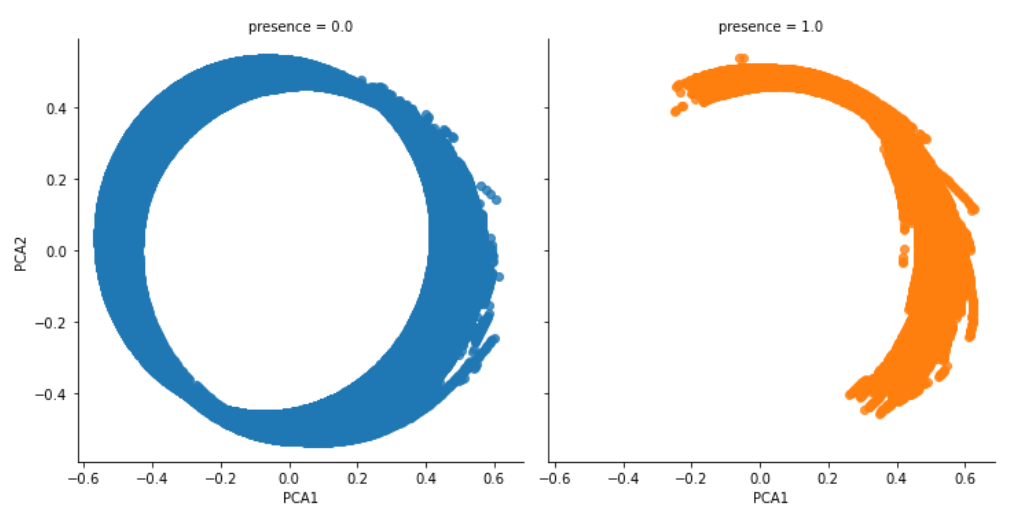
\includegraphics[width=0.85\textwidth]{pic/pca.png}
    \caption{Reduktion des Datensets auf zwei Dimensionen}
    \label{fig:pca}
\end{figure}

Die Menge der Anwesenheiten (orange) ist in \ref{fig:pca} nahezu identisch mit der rechten Teilmenge der 
Abwesenheiten (blau). 
Das heißt, dass alle Datenpunkte, die in der linken Hälfte des blauen Datensets liegen, sehr einfach klassifiziert 
werden können.\\
Legt man beide Datensets übereinander, ist es nun ohne die Einfärbung nahezu unmöglich zwischen An- und 
Abwesenheit zu unterscheiden.\\

\begin{figure}[h]
    \centering
    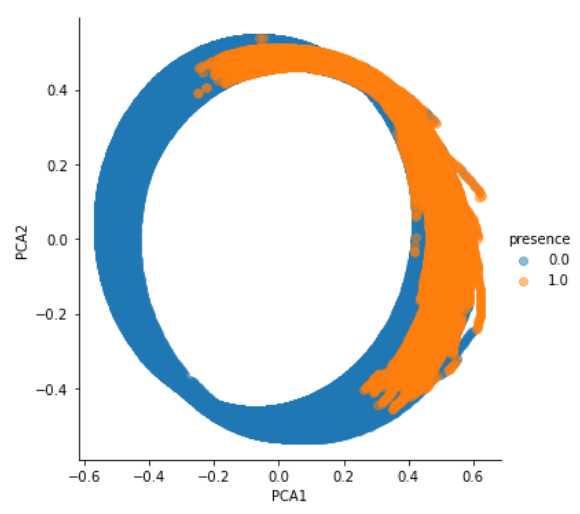
\includegraphics[width=0.5\textwidth]{pic/pca1.png}
    \caption{Datenreduktion ohne Trennung}
    \label{fig:pca1}
\end{figure}

Da die Datenpunkte im rechten Teilbild kaum zu unterscheiden sind, schafft es das Modell nicht, An- und Abwesenheit
während eines Arbeitstages zu unterscheiden. Währenddessen sind die Abwesenheiten im linken Teilbild sehr einfach
zu klassifizieren.
Diesen Sachverhalt spiegelt auch die Auswertung des \textit{Classification Report} in Tabelle \ref{tab:clus} wieder.\\

%Das Erkennen von Abwesenheit im linken Teilbild von \ref{fig:pca1} ist nun erheblich einfacher, als die Trennung 
%zwischen An- und Abwesenheit im rechten Teilbild. 
